\PassOptionsToPackage{svgnames}{xcolor}
\documentclass[a0paper]{betterposter}
\usepackage{tcolorbox}
\usepackage{lipsum}
\usepackage{hyperref}
\tcbuselibrary{skins,breakable}
\usetikzlibrary{shadings,shadows}

\newenvironment{beamerblock}[1]{%
    \tcolorbox[beamer,%
    noparskip,breakable,
    colback=LightBlue,colframe=DarkBlue,%
    colbacklower=DarkBlue!75!LightBlue,%
    title=#1]}%
    {\endtcolorbox}

% Better Poster latex template example v1.0 (2019/04/04)
% GNU General Public License v3.0
% Rafael Bailo
% https://github.com/rafaelbailo/betterposter-latex-template
% Original design from Mike Morrison
% https://twitter.com/mikemorrison

%% Setting the width of columns
% Left column
\setlength{\leftbarwidth}{0.191\paperwidth}
% Right column
\setlength{\rightbarwidth}{0.191\paperwidth}

%% Setting the column margins
% Horizontal margin
%\setlength{\columnmarginvertical}{0.05\paperheight}
% Vertical margin
%\setlength{\columnmarginhorizontal}{0.05\paperheight}
% Horizontal margin for the main column
%\setlength{\maincolumnmarginvertical}{0.15\paperheight}
% Vertical margin for the main column
%\setlength{\maincolumnmarginhorizontal}{0.15\paperheight}

%% Changing font sizes
% Text font
% \renewcommand{\fontsizestandard}{\fontsize{68}{72} \selectfont} %TODO
% Main column font
%\renewcommand{\fontsizemain}{\fontsize{28}{35} \selectfont}
% Title font
%\renewcommand{\fontsizetitle}{\fontsize{28}{35} \selectfont}
% Author font
%\renewcommand{\fontsizeauthor}{\fontsize{28}{35} \selectfont}
% Section font
%\renewcommand{\fontsizesection}{\fontsize{28}{35} \selectfont}

%% Changing colours
% Background of side columns
%\renewcommand{\columnbackgroundcolor}{black}
% Font of side columns
%\renewcommand{\columnfontcolor}{gray}
% Background of main column
%\renewcommand{\maincolumnbackgroundcolor}{empirical}
\renewcommand{\maincolumnbackgroundcolor}{theory}
%\renewcommand{\maincolumnbackgroundcolor}{methods}
%\renewcommand{\maincolumnbackgroundcolor}{intervention}
% Font of main column
%\renewcommand{\maincolumnfontcolor}{gray}

\begin{document}	

\newcommand{\ex}[1]{\textit{ #1 }}
\betterposter{ 
%main

\maincolumn{
    \begin{itemize}
        \item Gather images at a \textbf{single resource}.
        \item Establish a \textbf{common description framework} for image metadata.
        \item Provide \textbf{bulk, programmatic access} to image subsets.
    \end{itemize}
    }{
    \compactqrcode{img/git-logo_qrcode}{\texttt{github.com/ncar/rda-image-archive}}
    }


}{ 
%left

%header
\title{Towards\\ Categorical\\ Metadata\\ for Unreduced\\ Climate\\ Observations}
\author{Colton Grainger}
\institution{University of Colorado}

%content

%logos
\vfill
I am grateful for support from \textbf{SIParCS}, and for mentorship from \textbf{Thomas Cram}, \textbf{Matt~Mayernick}, and \textbf{Steve Worley}.\vspace{1em}
\begin{center}
    
\includegraphics[height=4.5em]{img/CISL-contemp-logo-blue-square}\hspace{0.5em}
    
\includegraphics[height=5em]{img/cu-logo}\hspace{0.5em}
    
\includegraphics[height=5em]{img/nsf-logo}
\end{center}

}{ 
%right

% tasks
\section{Status Quo}


    \begin{center}
        unreduced data from $\sim$100 Tb collection of images (ACRE)
    \end{center}


    \begin{beamerblock}{marine logbooks 1870--1950}
        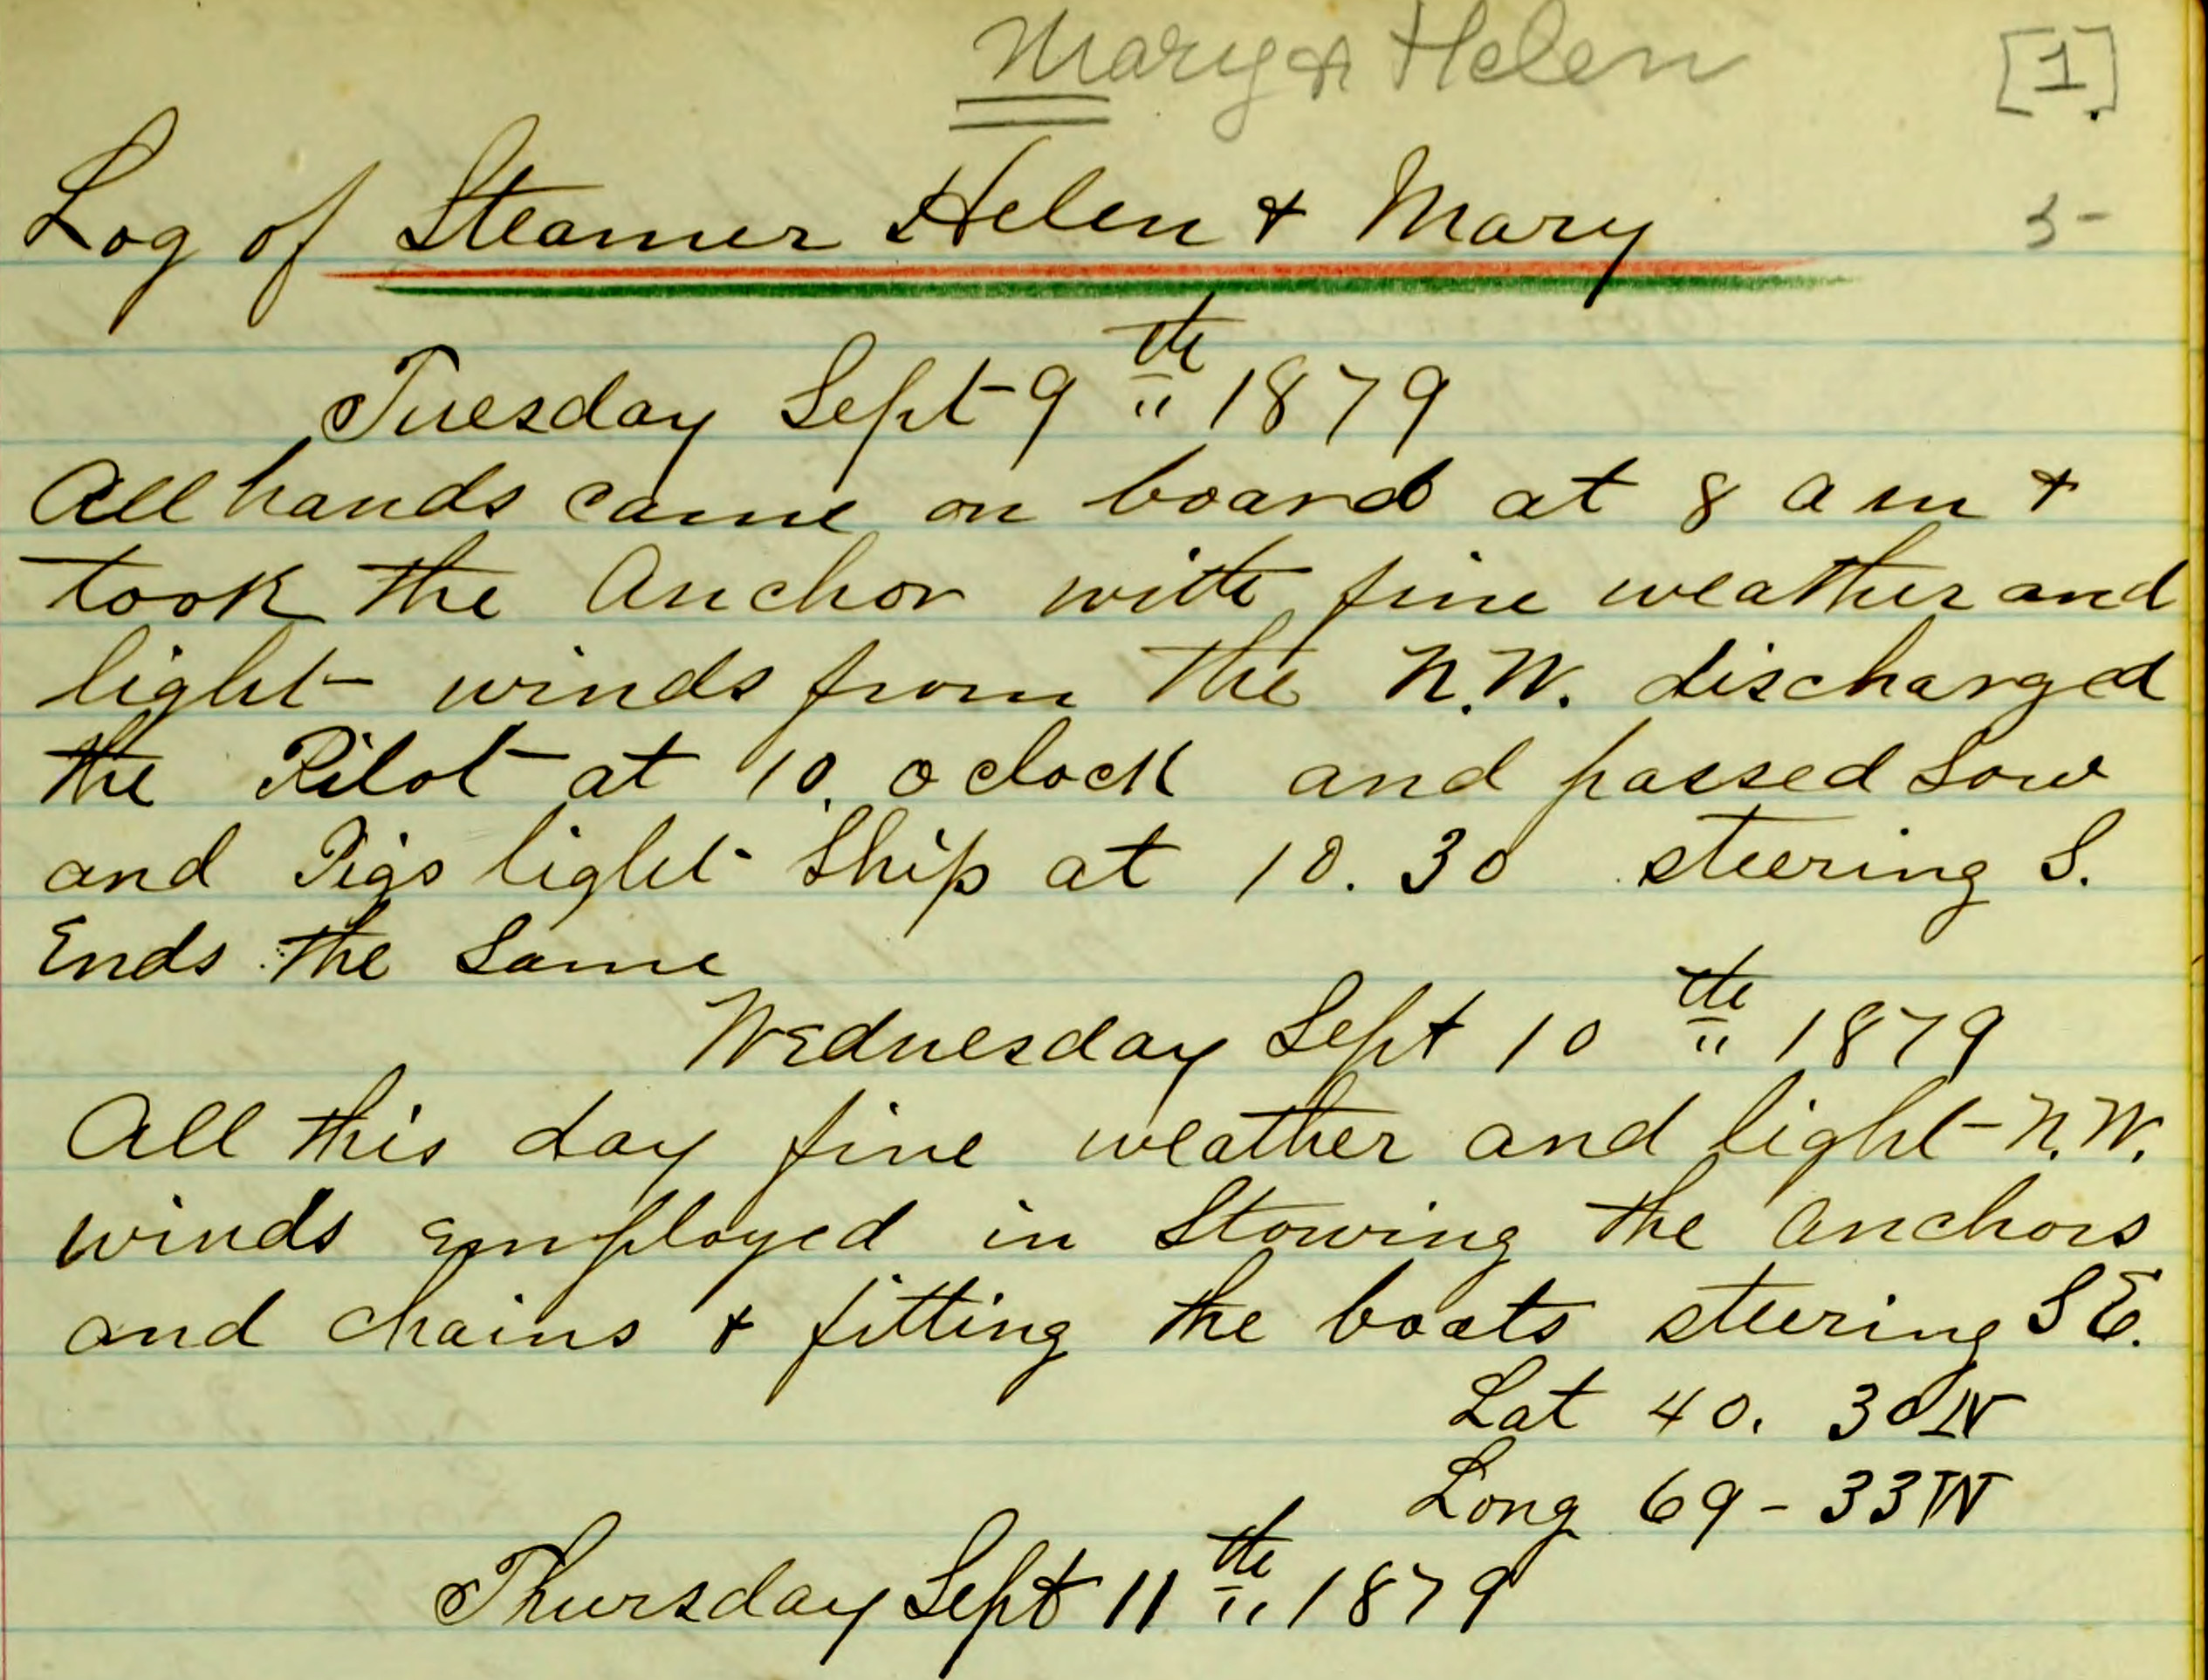
\includegraphics[height=12.5em]{img/mary-1879}
        \hspace{0.5em}
        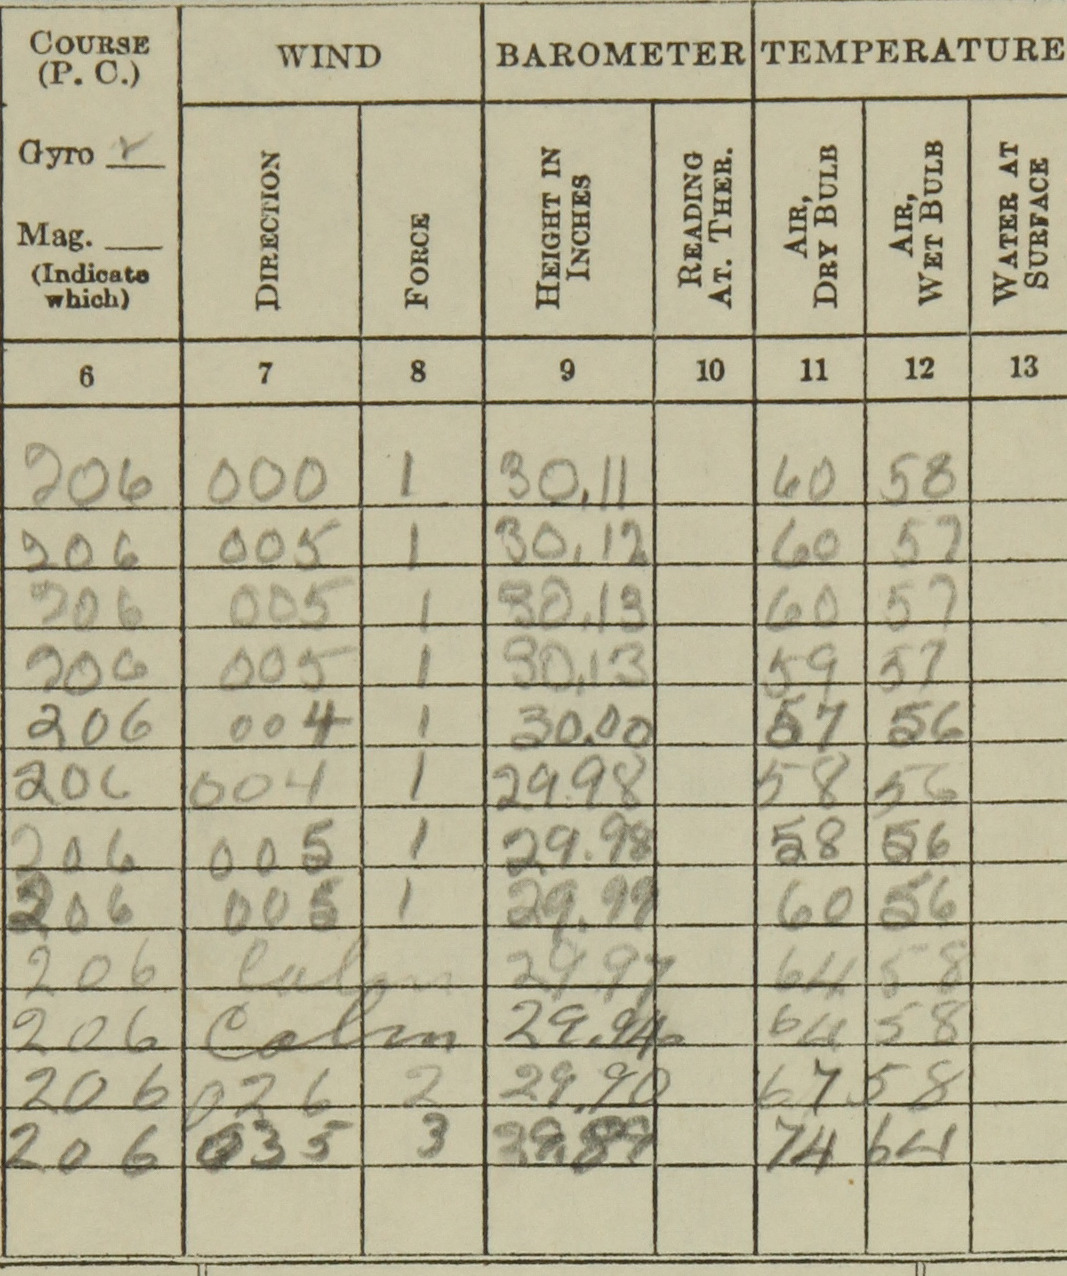
\includegraphics[height=12.5em]{img/idaho-1944}
    \end{beamerblock}
    \vfill

    \begin{beamerblock}{land stations 1870--1930}
        Indian Daily Weather Reports, Todd Folios, etc.
    \end{beamerblock}


    \ex{reduction of 6Mb image to a 2Kb time series}
        \begin{figure}
            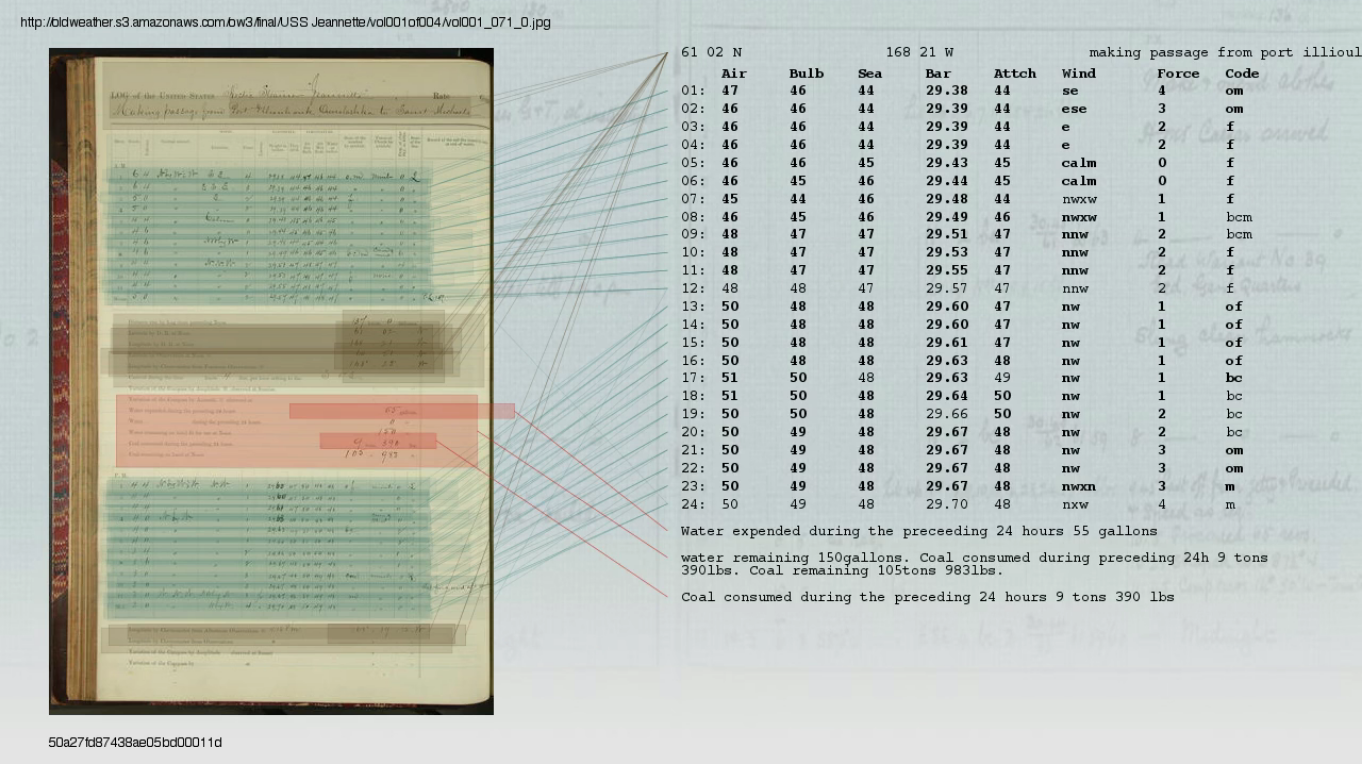
\includegraphics[width=\textwidth]{img/2019-07-30-jeannette}
            \caption{
                24 hours on the USS Jeannette (P. Brohan)
            }
        \end{figure}

  \begin{beamerblock}{\textit{url}}
        \url{twitter.com/NCAR\_RDA/status/1144058111654711296}
  \end{beamerblock}

  \begin{minipage}[t]{0.43\linewidth}
      \begin{figure}
      \textit{qrcode}
          
\includegraphics[width=\textwidth]{img/brohan_qrcode}
          \caption{
            \emph{CISL Seminar}, P.~Brohan (2019)
          }
      \end{figure}
  \end{minipage}
  \begin{minipage}[t]{0.55\linewidth}
      \ex
      \begin{itemize}
        \item $2^6$ bytes $\sim$ 70 ASCII characters
        \item $2^{12}$ bytes $\sim$ $441 \times 441$ pixels
        \item a \texttt{qrcode} \textbf{reduces} to a \texttt{url}
      \end{itemize}

\begin{verbatim}
\$ exiftool brohan_qrcode.png
File Size : 2.7 kB
Image Size : 441x441
MIME Type : image/png
\end{verbatim}
\end{minipage}

\section{Alternative}

  \begin{center}
    \textit{metadata}\\
    \texttt{\{'key:value' for key in <schema>\}}
  \end{center}
    \textit{what available metadata has low noise-to-signal ratio?}

\begin{minipage}[t]{0.5\linewidth}
    \begin{figure}
        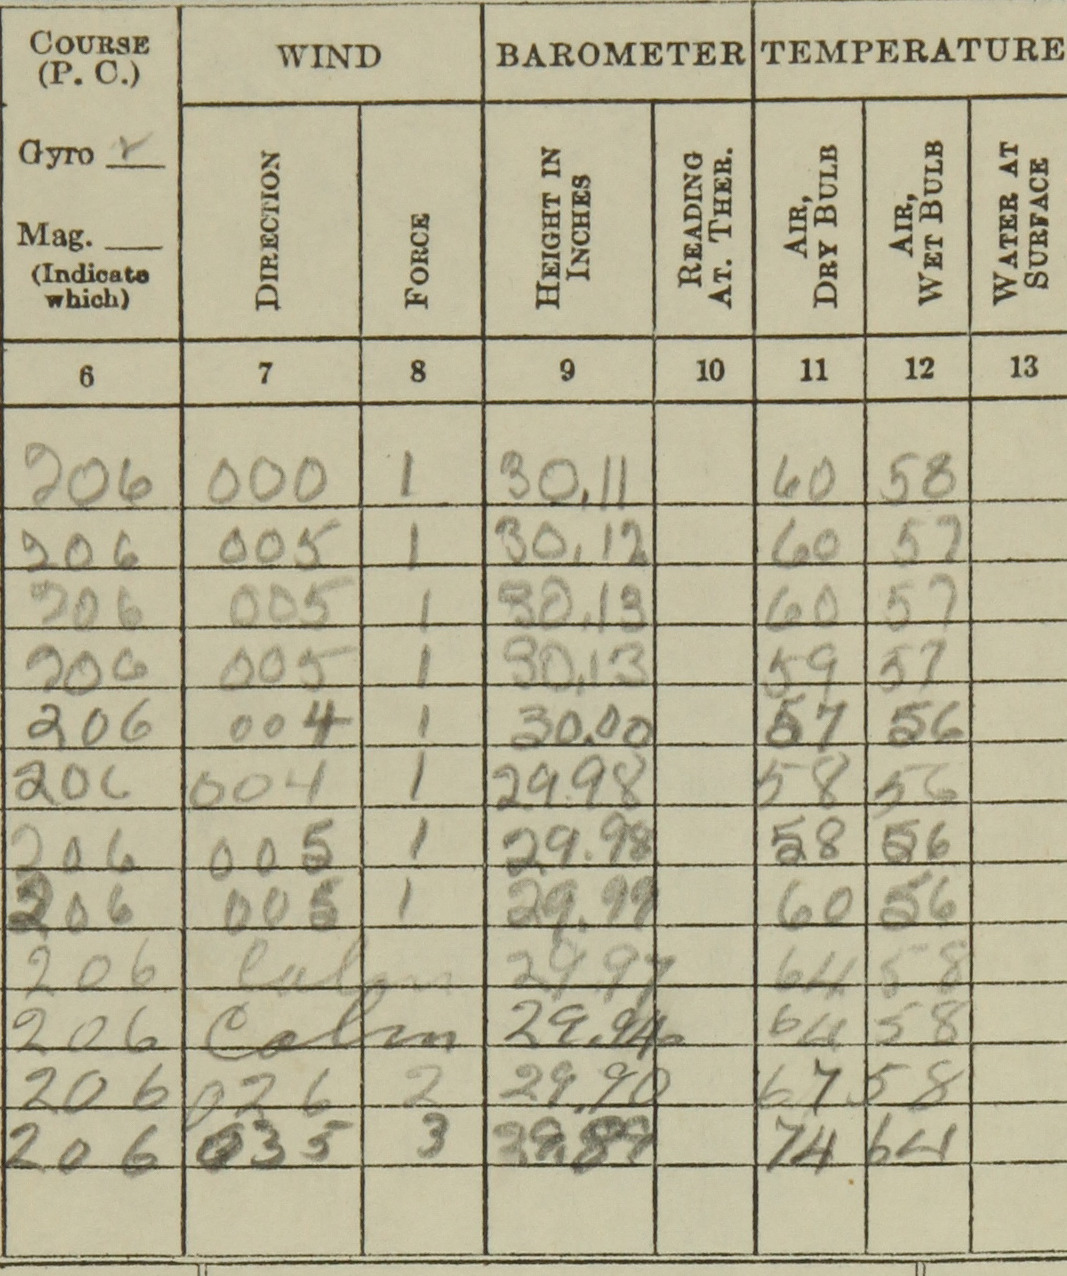
\includegraphics[width=0.9\textwidth]{img/idaho-1944}
        \caption{
            May 1944, Idaho (BB-42)
        }
    \end{figure}
\end{minipage}
%either math model or schema here TODO
\begin{minipage}[t]{0.45\linewidth}
\hspace{2em}
\begin{verbatim}
$ exiftool Idaho-BB-0034.JPG 
File Size : 4.6 MB
Image Size : 3744x5616
MIME Type : image/jpeg
\end{verbatim}
        \begin{description}
            \item[arc] archive
            \item[doc] document
            \item[img] image
            \item[obs] observation
            \item[plt] platform
        \end{description}
\end{minipage}

    \begin{itemize}
    \item Roughly, an image in the category $\text{img}$ approximates a time-series $\sigma \colon [t_0, t_1] \to \mathscr{S}$, where $\mathscr{S}$ is the state space of meteorological variables. 

    \item An observation is $\rho(t)$ evaluated at a time $t$.

    \item A platform in the category $\text{plt}$ approximates a time-series $\lambda \colon [t_0, t_1] \to M$, where $M$ is a differentiable manifold.
    \end{itemize}

    \begin{minipage}[t]{0.45\linewidth}
        \begin{description}
            \item[arc] archive
            \item[doc] document
            \item[img] image
            \item[obs] observation
            \item[plt] platform
        \end{description}
    \end{minipage}
    \begin{minipage}[t]{0.40\linewidth}
        \begin{block}{dependencies}
            $\xymatrix{
                \text{arc} \ar@{->>}[dr] &  & \ar@{->>}@/^5px/[dl] \text{plt} \\
                & \text{doc} \ar@{.>}@/^5px/[ur]^{\exists!} \ar@{->>}[dl] & \\
                \text{img} \ar@{->>}[rr] & & \text{obs} \ar@{_{(}->}[uu]_{\text{update}}}$
        \end{block}
    \end{minipage}

\subsection{3 Tasks}

    \begin{enumerate}
        \item Gather images into (at least) \textbf{one repository}. 
        \item Establish a \textbf{common description framework} for image metadata.
        \item Provide \textbf{bulk, programmatic access} to image subsets.
    \end{enumerate}

\subsection{Functions}

    \begin{description}
        \item[repo] MySQL schema with Makefile. \texttt{assign\_uuid()}.
        \item[framework] Agnostic ingest scripts.  Bundle metadata.
        \item[access] \texttt{rda.ucar.edu/i/<uuid>}
    \end{description}

\subsection{Interfaces}
    \begin{description}
        \item[repo] Conflict resolution for \texttt{assign-uuid()}.
        \item[framework] RELAX NG validator.
        \item[access] \texttt{rda.ucar.edu/i/<query>}
    \end{description}

\section{References}
    \begin{figure}
        
\includegraphics[width=0.5\textwidth]{img/git_qr.png}
        \caption{git repo}
    \end{figure}
\end{document}
\section{informal outline}
\begin{itemize}
\item
  introduction

  \begin{itemize}
  \tightlist
  \item
    to contextualize the project with reference to Kevin and Philip's
    work
  \end{itemize}
\item
  statement of problem and proposed solution
\item
  literature review

  \begin{itemize}
  \tightlist
  \item
    to distinguish the proposed solution from existing methods
  \item
    e.g., a survey of existing image repositories and archives
  \end{itemize}
\item
  summary of input from stakeholders

  \begin{itemize}
  \tightlist
  \item
    to list requirements, expected use cases, and design criteria
  \item
    to share comments from Philip, Kevin, and NCAR scientists
  \end{itemize}
\item
  case-study: implementing the proposed solution

  \begin{itemize}
  \tightlist
  \item
    subsections TBD
  \item
    likely to be divided chronologically,

    \begin{itemize}
    \tightlist
    \item
      e.g., metadata processing,
    \item
      data retrieval, \ldots{}
    \end{itemize}
  \end{itemize}
\item
  discussion

  \begin{itemize}
  \tightlist
  \item
    to abstract generalizable knowledge from the case-study
  \end{itemize}
\item
  future work
\item
  conclusion

  \begin{itemize}
  \tightlist
  \item
    with reference back to Kevin and Philip's work
  \end{itemize}
\item
  acknowledgements

  \begin{itemize}
  \tightlist
  \item
    mentors at NCAR
  \item
    visits from Philip and Kevin
  \end{itemize}
\item
  references

  \begin{itemize}
  \tightlist
  \item
    literature
  \item
    software
  \end{itemize}
\end{itemize}

} 

\end{document}
